\documentclass{article}

\usepackage{graphicx}
\usepackage[backend=biber,style=numeric]{biblatex}
\addbibresource{references.bib}
\usepackage[colorlinks=true, linkcolor=blue, urlcolor=blue, citecolor=blue, filecolor=blue]{hyperref}
\usepackage{amsmath}

\begin{document}
\title{Quantum Cryptography: Mid-Term Report}
\author{Harshil Solanki\\Roll number: 23B1016\\Mentor: Raunak Gupta}
\maketitle
\tableofcontents
\clearpage

\section{The Math}
Going deeper into Number Thoery has helped in building concepts very fundamentally (even some which are not currently needed). Of all I've read in \cite{numt} the topics I've found interesting is the studies involved in trying to find out the pattern of distribution of primes.

\subsection{Primes}
There is a clever way of identifying all primes lesser than a given integer $n$, {\it THE SIEVE OF ERATOSTHENES}. It works by picking up primes in line and eliminating it's multiples from the list till the prime is less than or equal to $\sqrt{n}$, leaving us with primes in the list.\\
Euclid proof that there exists infinite number of primes and the involved proving techniques turns out very important. For example, the theorem 
\begin{quote}
    If $p_n$ is the $n^{th}$ prime, then $p_n \leq 2^{2^{n-1}}$
\end{quote}
bounds primes using the Euclidean numbers and Induction.

\subsection{Congruence}
The notations and properties of Congruence turns out to be of massive importance to Cryptography. The Definition of Congruence goes like this:
\begin{quote}
    Let $n$ be a fixed positive integer. Two integers $a$ and $b$ are said to be {\it congruent modulo n}, symbolised by
    \begin{equation*}
        a \equiv b \pmod n
    \end{equation*}
    if $n$ divides the difference $a-b$; that is, provided that $a-b = kn$ for some integer $k$.
\end{quote}
It's comes with some interesting properties:
\begin{figure}[h]
    \centering
    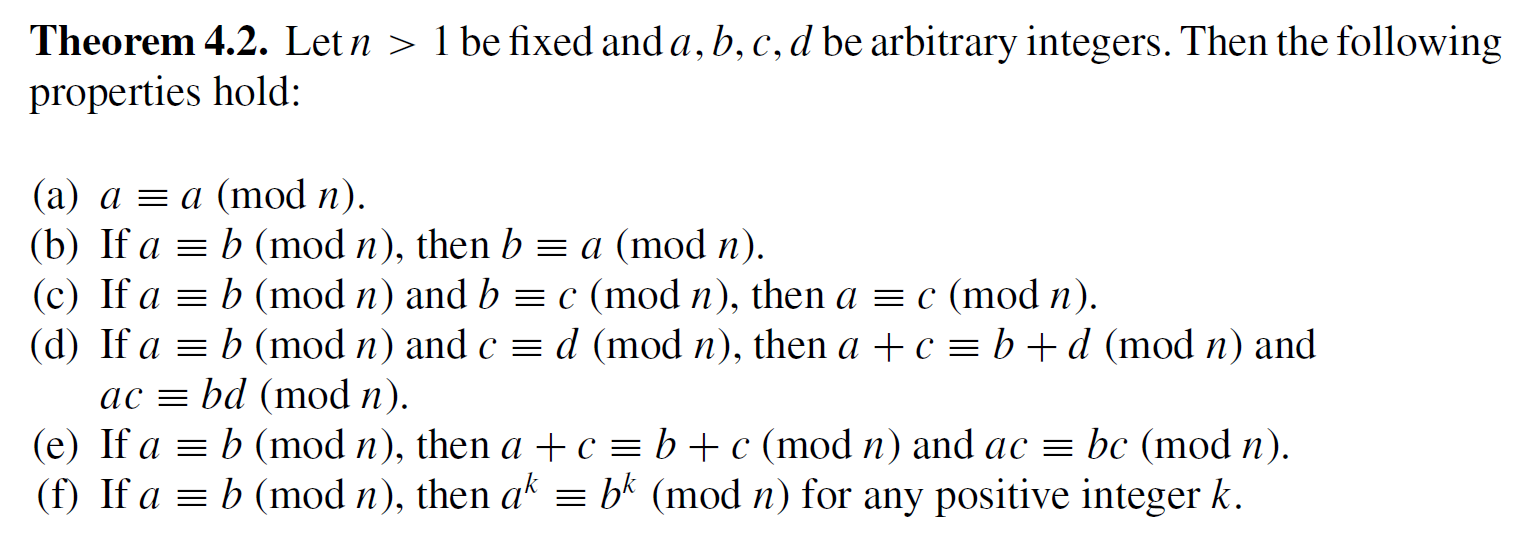
\includegraphics[width=\textwidth]{cong_prop.png}
    \caption{Some properties with Congruence \cite{cong_prop}}
    \label{fig:cong_prop}
\end{figure}

\subsection{Other Things}
Except these, history leads to various interesting theorems and concepts. Namely, Fermat's Theorem, {\it pseudoprimes} ($n$ such that $n |2^n-2$), Wilson's Theorem and Number-Theoretic functions.

\section{Introduction to Cryptography}

\subsection{Terminology}
\begin{itemize}
    \item[Cryptography]: (from the Greek {\it kryptos} meaning hidden and {\it graphein} meaning to write) The
    science of making communications unintelligible to all except authorized parties.
    \item[Plaintext]: The information to be concealed
    \item[Ciphertext]: The code
    \item[Encrypting]: The process of converting plaintext to ciphertext 
    \item[Decryption]: The process of converting ciphertext to plaintext
    \item[Cryptanalysis]: Study of techniques used for deciphering a message without any knowledge of the enciphering. Cryptanalysis is what the layperson calls “breaking the code.”
    \item[Brute-Force Attack] It involves trying every possible key until an intelligible translation of the ciphertext into plaintext is obtained
    \item[Perfect Secrecy] A cipher is said to achieve perfect secrecy if the knowledge of ciphertext messages does not alter the statistical distribution(the probability of decrypting) of the plaintext 
\end{itemize}

\subsection{Historical Ciphers}
\subsubsection{Caeser Cipher}
This method was used by the great Roman Emperor Julius Caeser around 50 {\small B.C.}.\\
It's a rudimentary substitution cipher in which each letter of the alphabet is replaced by the letter that occurs three places down the alphabet, with the last three letters cycled back to the first three letters.\\
\begin{figure}[h]
    \centering
    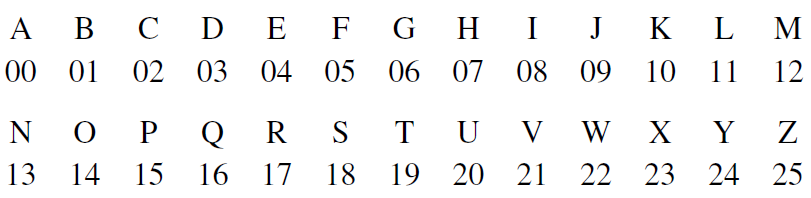
\includegraphics[width=\textwidth]{caeser.png}
    \caption{An example of correspondence between letters and digits in Caeser Cipher \cite{caeser}}
    \label{fig:caeser}
\end{figure}
If $P$ is the digital equivalent of a plaintext letter and $C$ is the digital equivalent of
the corresponding ciphertext letter, then
\begin{equation*}
    C \equiv P + 3 \pmod {26}
\end{equation*}
For example, a Caeser cipher for 
\begin{center}    
    CAESER WAS GREAT
\end{center}
is 
\begin{center}
    FDHVDU ZDV JUHDW
\end{center}

Such Encryption schemes in which the original message is replaced by the same cipher substitute are called {\it monoalphabetic ciphers}. These schemes turn out to be vulnerable as they can be easily decrypted using frequency analysis.\\
The frequency analysis works by comparing the relative frequency of letters with a standard frequency distribution for English. Further, instead of single letters, a block of two or more letters can also be analysed such way. If the message is long enough, this technique might be sufficient.

\subsubsection{Polyalphabetic Ciphers}
In such schemes, a plaintext letter has more than one ciphertext equivalents depending on it's position in the message.\\
A famous example of this scheme is given by a French cryptographer {\bf Blaise de Vigenere} (1523-1596). To implement this system, the communicating parties agree on an easily remembered word or phrase. With the standard alphabet numbered from $A = 00$ to $Z = 25$, the digital equivalent of the keyword is repeated as many times as necessary beneath that of the plaintext message. The message is then enciphered by adding, modulo 26, each plaintext number to the one immediately beneath it. The process may be illustrated with the keyword READY, whose numerical version is 17 04 00 03 24. Repetitions of this sequence are arranged below the numerical plaintext of the message
\begin{center}
    ATTACK AT ONCE
\end{center}
to produce the array
\begin{center}
    00 19 19 00 02 10 00 19 14 13 02 04\\
    17 04 00 03 24 17 04 00 03 24 17 04
\end{center}
When the columns are added modulo 26, the plaintext message is encrypted as
\begin{center}
    17 23 19 03 00 01 04 19 17 11 19 08
\end{center}
or, converted to letters,
\begin{center}
    RXTDAB ET RLTI
\end{center}
A weakness in Vigenere's approach is that once the length of the keyword has been determined, a coded message can be regarded as a number of separate monoalphabetic ciphers, each subject to straightforward frequency analysis.\\ \\
A clever modification that Vigenere contrived for his polyalphabetic cipher is currently called the {\it autokey} (“automatic key”). This approach makes use of the plaintext message itself in constructing the encryption key. The idea is to start off the keyword with a short seed or primer (generally a single letter) followed by the plaintext, whose ending is truncated by the length of the seed.\\
For example, assume that the message
\begin{center}
    ONE IF BY DAWN
\end{center}
is to be encrypted. Taking the letter K as the seed, the keyword becomes
\begin{center}
    KONEIFBYDAW
\end{center}
When both the plaintext and keyword are converted to numerical form, we obtain the array
\begin{center}
    14 13 04 08 05 01 24 03 00 22 13\\
    10 14 13 04 08 05 01 24 03 00 22
\end{center}
Adding the integers in matching positions modulo 26 yields the ciphertext
\begin{center}
    24 01 17 12 13 06 25 01 03 22 09
\end{center}
or, changing back to letters:
\begin{center}
    YBR MN GZ BDWJ
\end{center}

A way to ensure greater security in alphabetic substitution ciphers was devised in 1929 by {\bf Lester Hill}, an assistant professor of mathematics at Hunter College. Briefly, Hill's approach is to divide the plaintext message into blocks of n letters (possibly filling out the last block by adding “dummy” letters such as X's) and then to encrypt block by block using a system of n linear congruences in n variables.\\
In its simplest form, when $n = 2$, the procedure takes two successive letters and
transforms their numerical equivalents $P_1P_2$ into a block $C_1C_2$ of ciphertext
numbers via the pair of congruences
\begin{align*}
    C_1 \equiv aP_1 + bP_2 \pmod {26} \\
    C_2 \equiv cP_1 + dP_2 \pmod {26}
\end{align*}
To permit decipherment, the four coefficients $a, b, c, d$ must be selected so the $gcd(ad - bc, 26) = 1$.\\
In general terms, the Hill system can be expressed as
\begin{align*}
    C = E(K, P) &= PK \pmod {26}\\
    P = D(K, C) &= CK^{-1} \pmod {26} = PKK^{-1} = P
\end{align*}
where
\begin{quote}
    $P$ is the vector of plaintext letters in a block,\\
    $C$ is the vector of ciphertext letters in a block,\\
    $K$ is the Key,\\
    $E$ is the encryption scheme, and\\
    $D$ is the decryption scheme
\end{quote}
However, the key can be easily found if some plaintext-ciphertext pair is known in a message.

\subsubsection{Vernam's Cipher}
An influential nonalphabetic cipher was devised by Gilbert S. Vernam in 1917 while he was employed by the American Telephone and Telegraph Company (AT\&T). Vernam was interested in safeguarding information sent by the newly developed teletypewriter in which each letter was represented as a five digit binary code.\\
Any plaintext message such as
\begin{center}
    ACT NOW
\end{center}
would first be transformed into a sequence of binary digits:
\begin{center}
    110000111000001001100001111001
\end{center}
Vernam's innovation was to take as the encryption key an arbitrary sequence of 1's and 0's with length the same as that of the numerical plaintext. A typical key might appear as
\begin{center}
    101001011100100010001111001011
\end{center}
where the digits could be chosen by flipping a coin with heads as 1 and tails as 0.\\
Finally, the ciphertext is formed by adding modulo 2 the digits in equivalent places in the two binary strings.\\ The result in this instance becomes
\begin{center}
    011001100100101011101111110010
\end{center}
A crucial point is that the intended recipient must possess in advance the encryption key, for then the numerical plaintext can be reconstructed by merely adding modulo 2 corresponding digits of the encryption key and ciphertext.\\ \\
{\it {\bf Note:} In the early applications of Vernam's telegraph cipher, the keys were written on numbered sheets of paper and then bound into pads held by both correspondents. A sheet was torn out and destroyed after its key had been used just once. For this reason, the Vernam enciphering procedure soon became known as the one-time system or one-time pad. It achieves perfect secrecy.}

\subsection{Stream Cipher}
Stream ciphers are well-studied cryptographic primitives that somehow mimic the one-time pad, while using only a small secret key. For simplicity, we restrict ourselves to synchronous stream ciphers. The idea is to generate
a long keystream $Z = (z_i), i \in \{0\dots N - 1\}$, from a secret key $K \in \mathbf{Z}^n_2$,
where $N \gg n$, using a pseudo-random expansion function. The generated keystream can then be used to encrypt the plaintext, bit per bit, in a fashionidentical to the one-time pad: $c_i = p_i \oplus z_i$. Although the size $n$ of the key
typically ranges between 128 and 256 bits, the keystream can be used to
encrypt gigabytes of data.

\section{Symmetric Key Cryptography}
\begin{figure}[h]
    \centering
    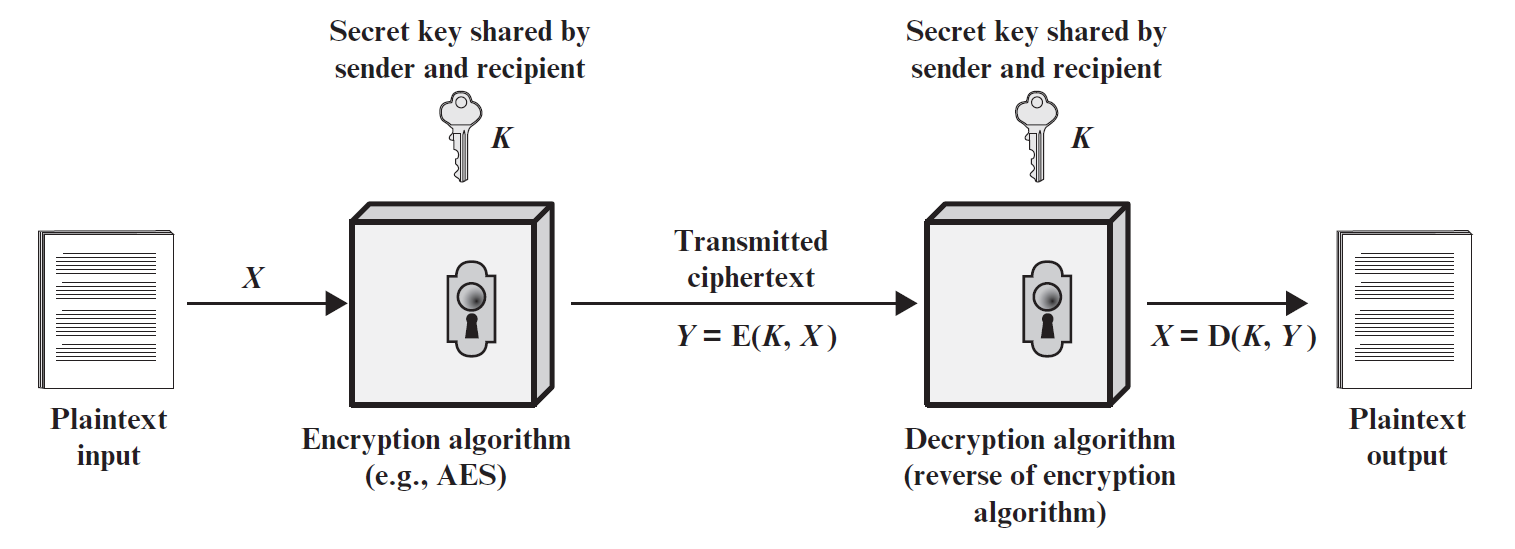
\includegraphics[width=\textwidth]{symkey.png}
    \caption{Simple Illustration of Symmetric Encryption \cite{symkey}}
    \label{fig:symkey}
\end{figure}
All Historical Ciphers mentioned have Symmetric Encryption scheme. This scheme focuses solely on having a single key for encryption and decryption of the message.\\

\subsection{Playfair Cipher}
The best-known multiple-letter encryption cipher is the Playfair, which treats digrams (frequency of two-letter combinations) in the plaintext as single units and translates these units into ciphertext digrams.\\
The working of this technique is illustrated by an example in \cite{playfair}: Figure~\ref{fig:playfair}
Nevertheless it uses a stronger encryption scheme than Caser Cipher, it keeps the structure of the message simple enough for a cryptanalyst to tackle down, which can b done by tracking the relative frequencies of letters.
\begin{figure}[h]
    \centering
    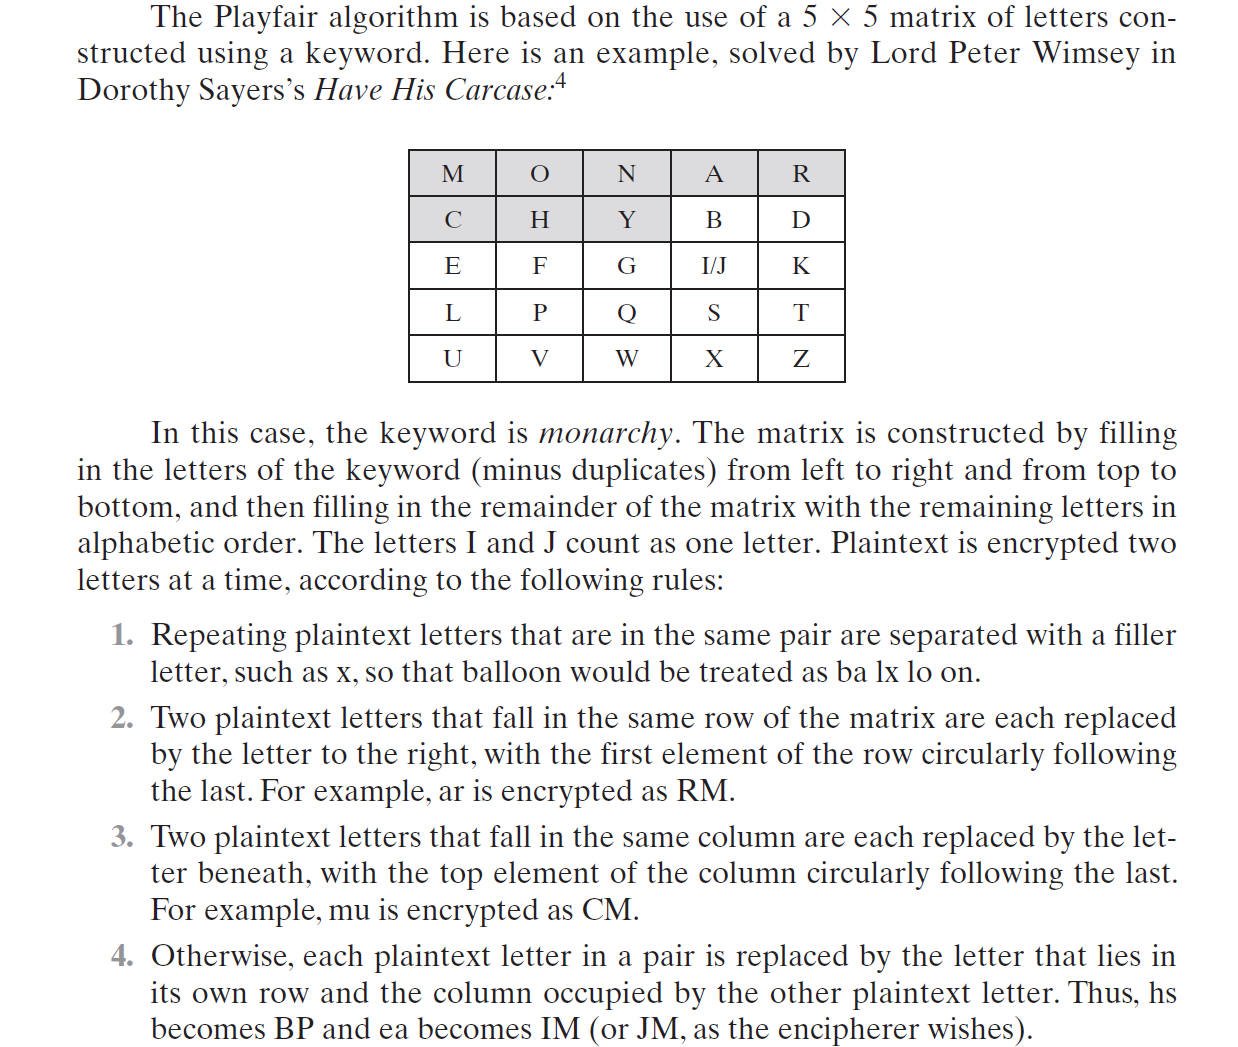
\includegraphics[width=\textwidth]{playfair.png}
    \caption{An example of implementing Playfair Cipher}
    \label{fig:playfair}
\end{figure}

The techniques discussed above so far involve substitution of a ciphertext symbol for a plaintext symbol. A very different kind of mapping is achieved by performing some sort of permutation on the plaintext letters. This technique is referred to as a
transposition cipher.

\subsection{Transposition Cipher}
The simplest such cipher is the {\bf rail fence} technique, in which the plaintext is written down as a sequence of diagonals and then read off as a sequence of rows. A more complex scheme is to write the message in a rectangle, row by row, and read the message off, column by column, but permute the order of the columns. The order of the columns then becomes the key to the algorithm.\\
A way to make the encryption stronger is to use double transposition instead of a single one.

\subsection{Rotor Machines}
This essentially generates a large amount of polyalphabetic substitution ciphers with 26 * 26 * 26 = 17,576 different substitution alphabets (for 3-motor machine Figure~\ref{fig:rotors}) used before the system repeats. Making a 5-motor machine equivalent to Vigenere cipher with a key length of 11,881,376.\\
With each stroke the first motor rotates one step changing the mapping of alphabets in the first motor itself, subsequent motors rotate one step on a complete rotation of the previous motor.\\
The technique turns out formidable be solved by using frequency analysis. 
\begin{figure}[h]
    \centering
    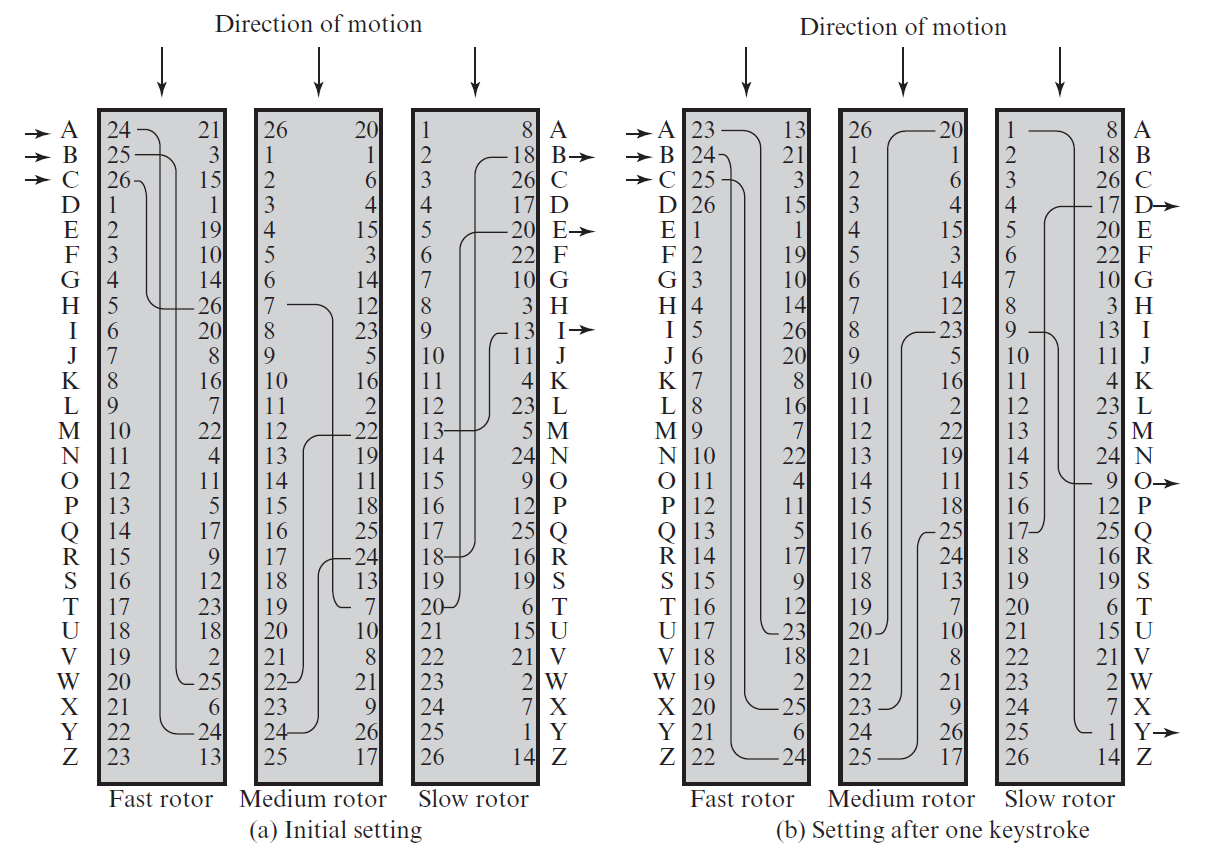
\includegraphics[width=\textwidth]{rotors.png}
    \caption{Three-Rotor Machine with Wiring Represented by Numbered Contacts \cite{rotors}}
    \label{fig:rotors}
\end{figure}

\subsection{FEISTEL CIPHER STRUCTURE} 
The left-hand side of Figure \ref{fig:feistel} depicts the encryption structure proposed by Feistel. The inputs to the encryption algorithm are a plaintext
block of length $2w$ bits and a key $K$. The plaintext block is divided into two halves,
$LE_0$ and $RE_0$. The two halves of the data pass through n rounds of processing and
then combine to produce the ciphertext block. Each round $i$ has as inputs $LE_{i-1}$ and
$RE_{i-1}$ derived from the previous round, as well as a subkey $K_i$ derived from the overall
$K$. In general, the subkeys $K_i$ are different from $K$ and from each other. In Figure
\ref{fig:feistel}, 16 rounds are used, although any number of rounds could be implemented.
All rounds have the same structure. A substitution is performed on the left
half of the data. This is done by applying a round function $F$ to the right half of the
data and then taking the exclusive-OR of the output of that function and the left
half of the data. The round function has the same general structure for each round
but is parameterized by the round subkey $K_i$. Another way to express this is to say
that $F$ is a function of right-half block of $w$ bits and a subkey of $y$ bits, which produces
an output value of length $w$ bits: $F(RE_i, K_{i+1})$. Following this substitution, a
permutation is performed that consists of the interchange of the two halves of the
data. This structure is a particular form of the substitution-permutation network
(SPN) proposed by Shannon.

\begin{figure}[h]
    \centering
    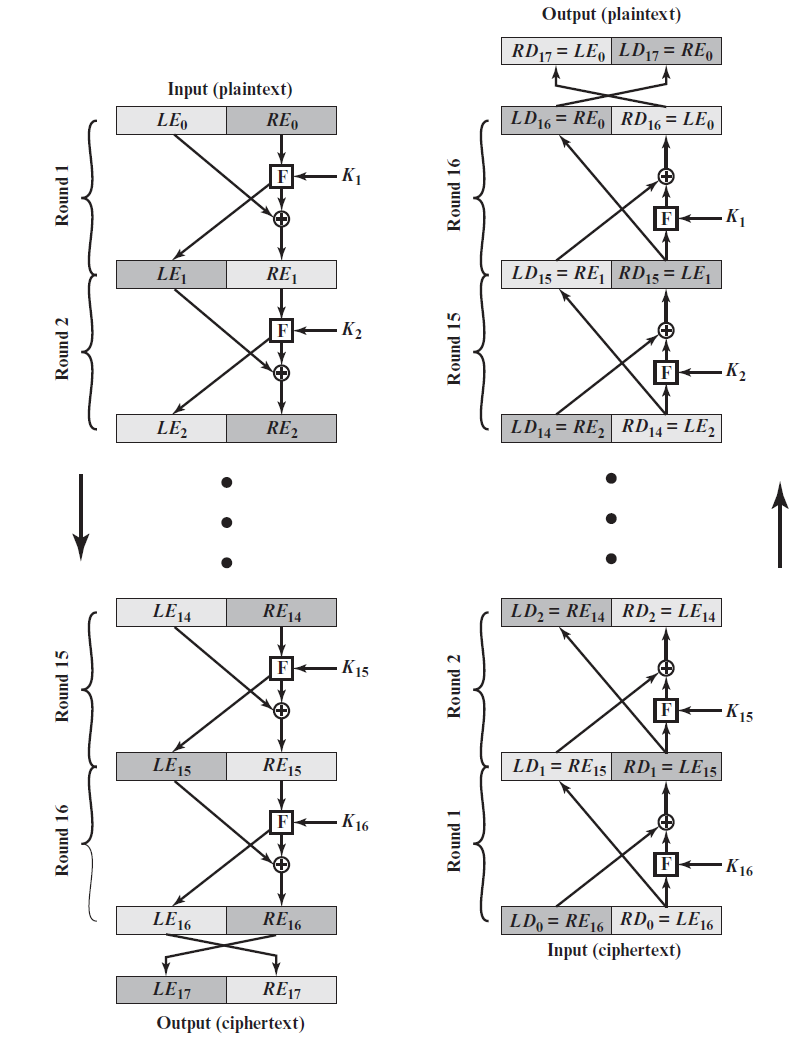
\includegraphics[width=\textwidth]{feistel.png}
    \caption{Feistel Encryption and Decryption \cite{feistel}}
    \label{fig:feistel}
\end{figure}

\subsection{The Data Encryption Standard}
The overall scheme for DES encryption is illustrated in Figure \ref{fig:des}. As with any
encryption scheme, there are two inputs to the encryption function: the plaintext to
be encrypted and the key. In this case, the plaintext must be 64 bits in length and the
key is 56 bits in length.\\
Looking at the left-hand side of the figure, we can see that the processing
of the plaintext proceeds in three phases. First, the 64-bit plaintext passes through
an initial permutation ($IP$) that rearranges the bits to produce the permuted input.
This is followed by a phase consisting of sixteen rounds of the same function, which
involves both permutation and substitution functions. The output of the last (sixteenth)
round consists of 64 bits that are a function of the input plaintext and the
key. The left and right halves of the output are swapped to produce the preoutput.
Finally, the preoutput is passed through a permutation [$IP^{-1}$] that is the inverse of
the initial permutation function, to produce the 64-bit ciphertext. \\
With the exception of the initial and final permutations, DES has the exact structure of a Feistel
cipher, as shown in Figure \ref{fig:feistel}.
The right-hand portion of Figure \ref{fig:des} shows the way in which the 56-bit key is
used. Initially, the key is passed through a permutation function. Then, for each of
the sixteen rounds, a subkey ($K_i$) is produced by the combination of a left circular
shift and a permutation. The permutation function is the same for each round, but a
different subkey is produced because of the repeated shifts of the key bits.\\\\

\begin{figure}[!h]
    \centering
    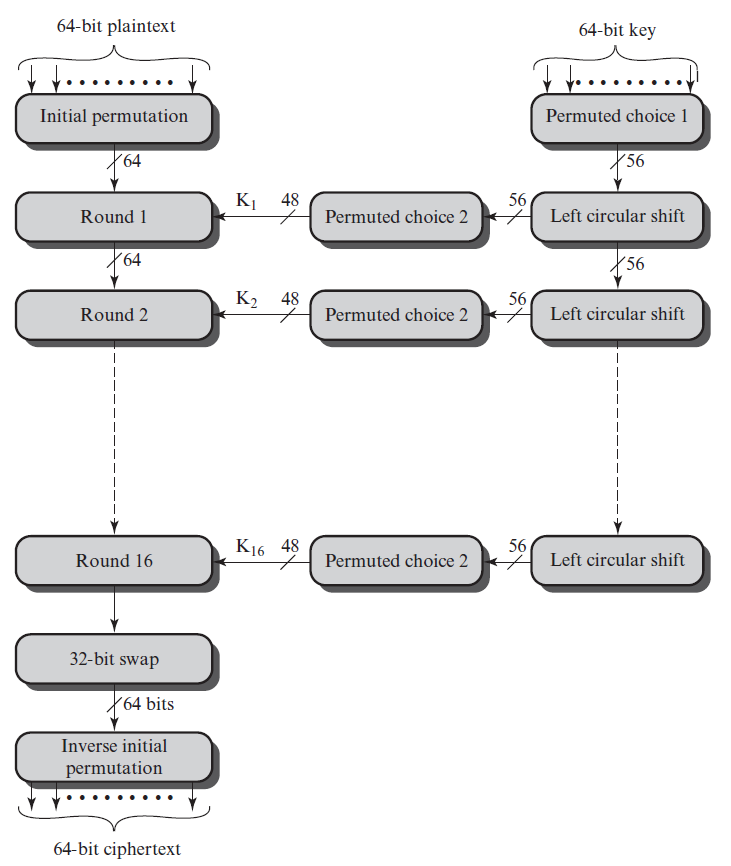
\includegraphics[width=\textwidth]{des.png}
    \caption{General Description of DES Encryption Algorithm \cite{des}}
    \label{fig:des}
\end{figure}

The concept of Advanced Encryption Standard will be dealt later in depth, according to PoA.

\section{Assymmetric Key Cryptography}
Figure \ref{fig:pubkey} outlines the working of Assymmetric Key/ Public Key Cryptosystems.

\subsection{Terminology}
\begin{itemize}
    \item[Asymmetric Keys] Two related keys, a public key and a private key, that are used to perform complementary operations, such as encryption and decryption or signature generation and signature verification.
    \item[Public Key Certificate] A digital document issued and digitally signed by the private key of a Certification Authority that binds the name of a subscriber to a public key. The certificate indicates that the subscriber identified in the certificate has sole control and access to the corresponding private key.
    \item[Public Key Infrastructure (PKI)] A set of policies, processes, server platforms, software and workstations used for the purpose of administering certificates and public-private key pairs, including the ability to issue, maintain, and revoke public key certificates.
\end{itemize}

\begin{figure}[!h]
    \centering
    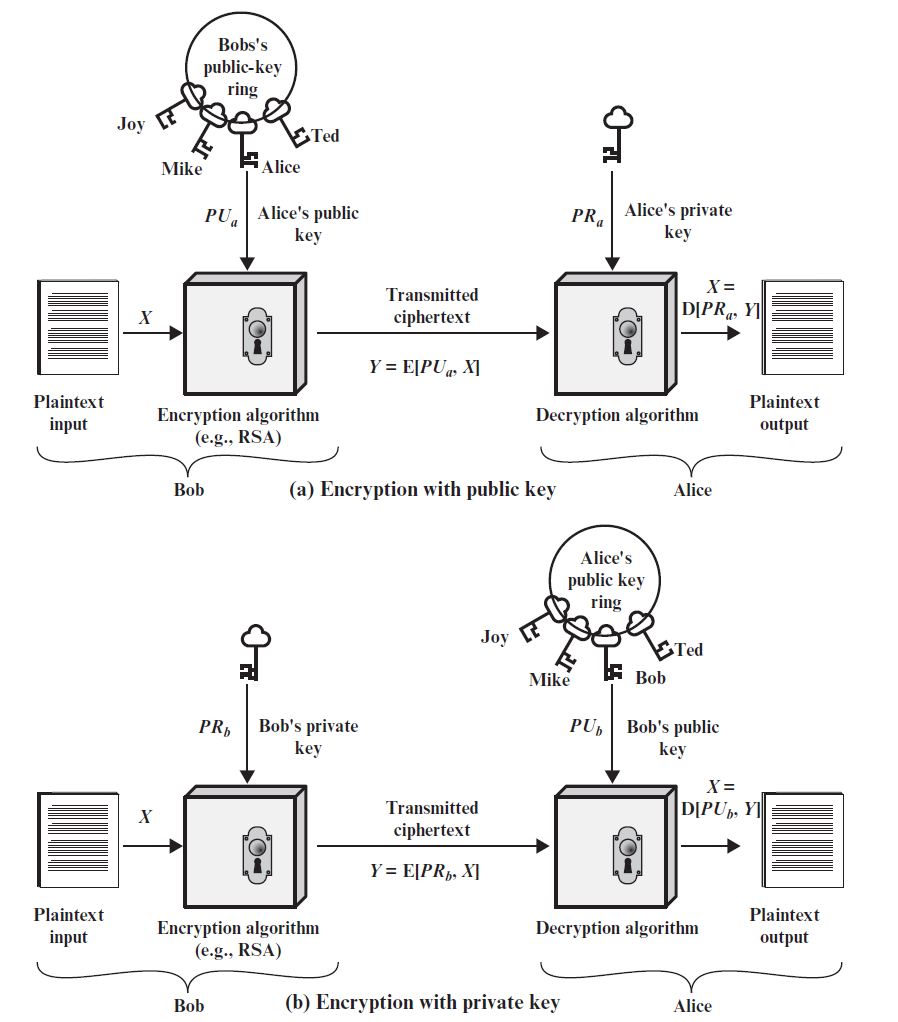
\includegraphics[width=\textwidth]{publickey.png}
    \caption{Public-Key Cryptography \cite{pubkey}}
    \label{fig:pubkey}
\end{figure}

In case A prepares a message to B and encrypts it using A's private key then B can decrypt the message using A's public key. Because the
message was encrypted using A's private key, only A could have prepared the message.
Therefore, the entire encrypted message serves as a {\bf digital signature}. In addition,
it is impossible to alter the message without access to A's private key, so the
message is authenticated both in terms of source and in terms of data integrity.\\

{\bf Note:} In general, we can say a problem is {\it infeasible} if the effort to solve it grows
faster than polynomial time (if the length of the input is $n$ bits, then the
time to compute the function is proportional to $n^a$, where $a$ is a fixed constant) as a function of input size.

\subsection{The Rivest-Shamir-Adleman (RSA) Algorithm}
RSA makes use of an expression with exponentials. Plaintext is encrypted in blocks,
with each block having a binary value less than some number $n$. That is, the block
size must be less than or equal to $log_2(n) + 1$; in practice, the block size is $i$ bits,
where $2^i < n \leq 2^{i+1}$. Encryption and decryption are of the following form, for
some plaintext block $M$ and ciphertext block $C$.
\begin{align}
    C &= M^e \pmod n\\
    M &= C^d \pmod n = (M^e)^d \pmod n = M^{ed} \pmod n
\end{align}
Both sender and receiver must know the value of $n$. The sender knows
the value of $e$, and only the receiver knows the value of $d$. Thus, this is a publickey
encryption algorithm with a public key of $PU = \{e, n\}$ and a private key of
$PR = \{d, n\}$. For this algorithm to be satisfactory for public-key encryption, the following
requirements must be met.
\begin{enumerate}
    \item  It is possible to find values of $e, d,$ and $n$ such that $M^{ed} \pmod n = M$ for all $M < n$.
    \item  It is relatively easy to calculate $M^e \pmod n$ and $C^d \pmod n$ for all values of $M < n$.
    \item  It is infeasible to determine $d$ given $e$ and $n$.
\end{enumerate}

The Algorithm can be depicted by Figure~\ref{fig:rsa}\\\\
The RSA Algorithm heavily relies on the computational inefficiency for factoring large numbers into prime, however quantum computers-computers that operate on the principles of quantum mechanics-can break standard RSA cryptosystem
via the celebrated Shor's quantum algorithm for efficient factoring.

\begin{figure}[!h]
    \centering
    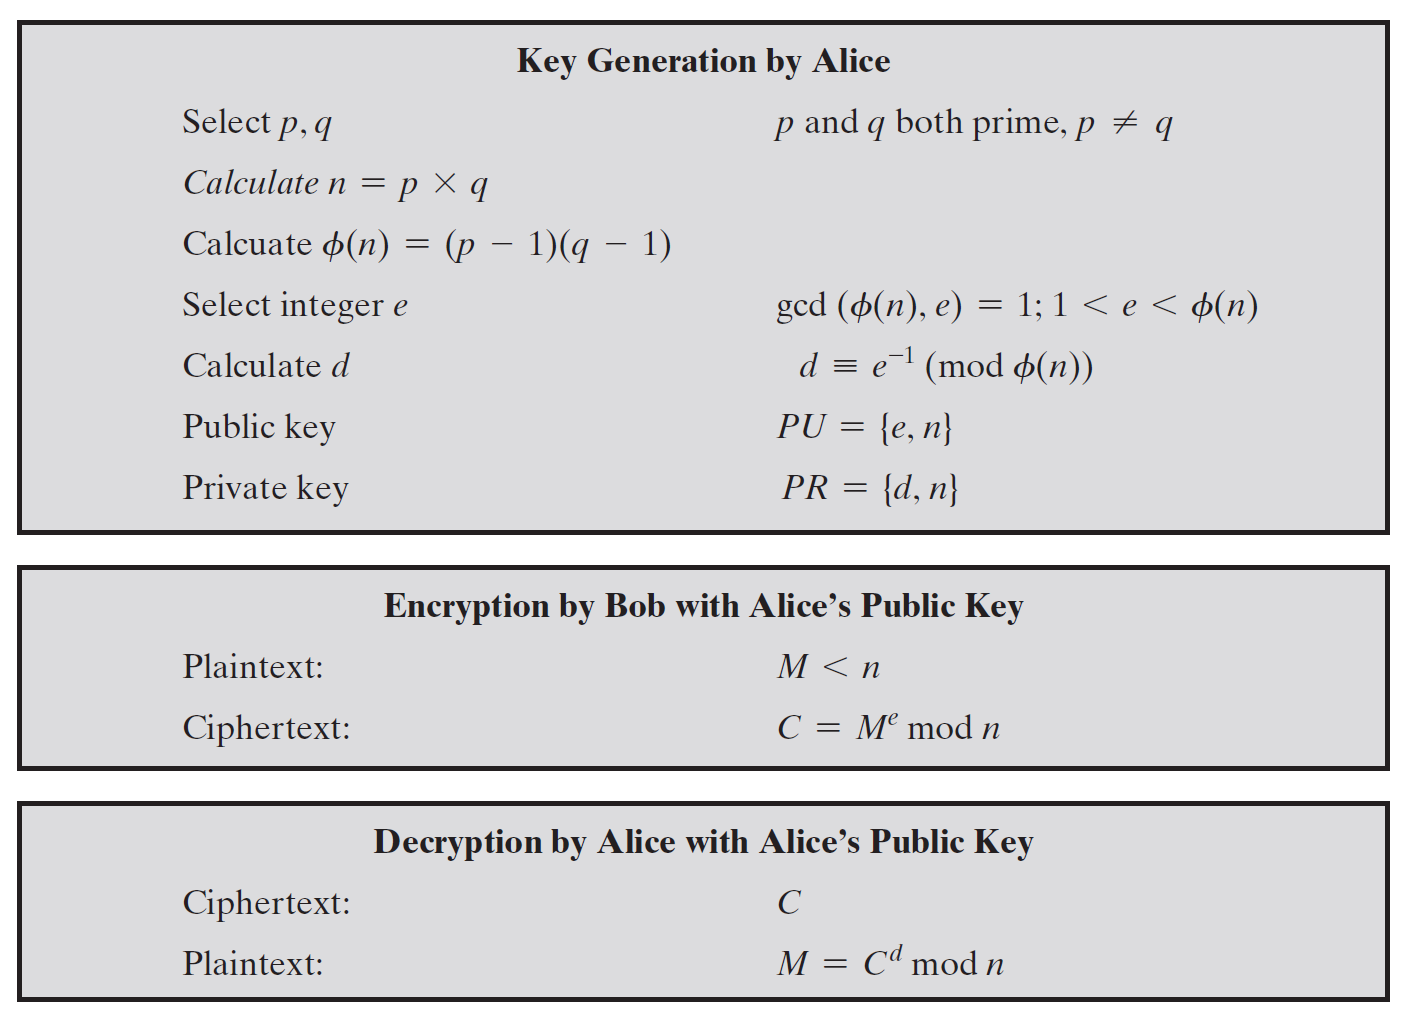
\includegraphics[width=\textwidth]{rsa.png}
    \caption{The RSA Algorithm \cite{rsa}}
    \label{fig:rsa}
\end{figure}

\section{Cryptographic Hash Functions}
A hash function $H$ accepts a variable-length block of data $M$ as input and produces
a fixed-size hash value $h = H(M)$. A “good” hash function has the property that the
results of applying the function to a large set of inputs will produce outputs that are
evenly distributed and apparently random. In general terms, the principal object of
a hash function is data integrity. A change to any bit or bits in $M$ results, with high
probability, in a change to the hash value.\\
Commonly, message authentication is achieved using a message
authentication code (MAC), also known as a keyed hash function. Typically, MACs
are used between two parties that share a secret key to authenticate information
exchanged between those parties. A MAC function takes as input a secret key and
a data block and produces a hash value, referred to as the MAC, which is associated
with the protected message.\\
When a hash function is used to provide message authentication,
the hash function value is often referred to as a {\bfseries message digest}.

\subsection{Digital Signatures}
Hash Functions can be used as Digital Signatures. The sender encrypts the message digest created by the original message using their private key and attaches the digest at the end of the message. The recipient computes their own hash value using the message and compares it to the digest attached to the message by decrypting it using the sender's public key. This process insures the integrity of the message. An attacker cannot alter the Hash code attached to the message without the knowledge of the sender's private key.

\subsection{Password Protection}
Hash Functions are commonly used to create {\it One-Way password files}. The Operating System stores the Hash of a password instead of storing the password directly making the password un-reachable by a hacker who gains access to the password file. When a user tries to login, the hash of the entered password is compared to the stored hash to authenticate.\\
Other uses of Hash functions include {\it intrusion detection} and {\it virus detection} which comprises of storing hash of the complete file and generating hash of current file to see whether the file is changed or not.

\subsection{SHA-512 (Secure Hash Algorithm)}
The algorithm takes as input a message with a maximum length of less than $2^{128}$ bits and produces as output a 512-bit message digest. The input is processed in 1024-bit blocks.\\
The Algorithm, in simple words, goes as follows:\\
\begin{enumerate}
    \item The Message is padded with a string of bits, where the first bit is 1 and others are 0, and an unsigned 128-bit integer containing the length of the original message, until the total length of the message becomes a multiple of 1024.
    \item A 512-bit buffer is initialised to hold the intermediate and final results of the hash function. This buffer can be viewed as eight 64-bit registers which contain the first 64-bits of the fractional parts of the square roots of the first eight prime numbers.
    \item Processing each block includes an 80 round module where in each round the value of a register is shifted right. The leftmost register gets it's value by as a function of the values of all previous registers except the fourth register. The new value of the fifth register is a function of fourth to eighth registers instead of being copied from the previous fourth register.
    \item The Output from the last stage (the stage in which there is no more message block left to process) is the 512-bit digest.
\end{enumerate}

\section{Quantum Cryptography}
\subsection{The Need}
The goal of quantum cryptography
is to perform tasks that are impossible or intractable with conventional cryptography. Quantum
cryptography makes use of the subtle properties of quantum mechanics such as the quantum
no-cloning theorem and the Heisenberg uncertainty principle. Unlike conventional cryptography,
whose security is often based on unproven computational assumptions, quantum cryptography
has an important advantage in that its security is often based on the laws of physics. Thus far,
proposed applications of quantum cryptography include quantum key distribution (abbreviated
QKD), quantum bit commitment and quantum coin tossing. These applications have varying
degrees of success. The most successful and important application—QKD—has been proven to be
unconditionally secure. Moreover, experimental QKD has now been performed over hundreds of
kilometers over both standard commercial telecom optical fibers and open-air. In fact, commercial
QKD systems are currently available on the market.~\cite{lo2008quantumcryptography}

\subsection{Overview of Quantum Key Distribution}
The Understanding of QKD can be illustrated by a simplified description of the first QKD protocol, created by Bennett and Brassard in 1984, called BB84 for short~\cite{Bennett_2014}.

\subsubsection{BB84}


\clearpage
\printbibliography

\end{document}